\documentclass{IFES-beamer}
\usepackage{pgfplots}
\pgfplotsset{compat=1.15}
\usepackage{amssymb}
\usepackage{graphicx,xcolor}
\usepackage{color}
\definecolor{ccqqqq}{rgb}{1,0,0}
\definecolor{darkGreen}{rgb}{0,.5,0}


%%%%%%%%%%%%%%%%%%%%%%%%%%%%%%%%%%%%
%  Defini o estlo no algorithmic
%%%%%%%%%%%%%%%%%%%%%%%%%%%%%%%%%%%%%
\newcommand{\red}{\color{red}}
\newcommand{\green}{\color{green}}
\newcommand{\TODO}[1]{{{\red #1}}}
\newcommand{\var}[1]{\text{#1}} %define estilo de nomes de variaveis
\newcommand{\defi}[1]{\textbf{#1}} % defini estilo ao definir algo no texto
\def\Nil{\text{NIL}}

\newcommand\circledmark{%
  \ooalign{%
    \hidewidth
    \kern-0.4ex\raisebox{-2.1ex}{\scalebox{5.5}{\textcolor{darkGreen}{\textbullet}}}
    \hidewidth\cr
    \kern-.6ex\raisebox{.6ex}{\color{white}$\checkmark$}\cr
  }%
}
\newcommand\custommark{%
  \ooalign{%
    \hidewidth
    \kern-0.4ex\raisebox{-2.1ex}{\scalebox{5.5}{\textcolor{white}{\textbullet}}}
    \hidewidth\cr
    \kern-.6ex{\color{black}$\checkmark$}\cr
  }%
}


\usepackage[Algoritmo]{algorithm}
\usepackage[noend]{algpseudocode}
\algrenewcommand\algorithmicif{\textbf{se}}
\algrenewcommand\algorithmicfor{\textbf{para}}
\algrenewcommand\algorithmicelse{\textbf{senão}}
\algrenewcommand\algorithmicwhile{\textbf{enquanto}}
\algrenewcommand\algorithmicdo{\textbf{faça}}
\algrenewcommand\algorithmicend{\textbf{fim}}
\algrenewcommand\algorithmicthen{\textbf{então}}
\algrenewcommand\algorithmicreturn{\textbf{retorne}}

%%%%%%%%%%%%%%%%%%%%%%%%%%%%%%%%%%%%%
% Comandos de notação assintotica   %
%%%%%%%%%%%%%%%%%%%%%%%%%%%%%%%%%%%%%
\renewcommand{\O}[1]{\text{O}(#1)}
\newcommand{\OTheta}[1]{\Theta(#1)}

%%%%%%%%%%%%%%%%%%%%%%%%%%%%%%
%     Métodos de Grafos      %
%%%%%%%%%%%%%%%%%%%%%%%%%%%%%%
\newcommand{\graphCreate}{\AlgoName{novoGrafo}}
\newcommand{\graphAdd}{\AlgoName{ligueGLA}}
\newcommand{\graphDel}{\AlgoName{removaGLA}}

%%%%%%%%%%%%%%%%%%%%%%%%%%%%%%
%     Métodos de Treap       %
%%%%%%%%%%%%%%%%%%%%%%%%%%%%%%
\newcommand{\treapCreate}{\AlgoName{novoNó}}
\newcommand{\treapSearch}{\AlgoName{busca}}
\newcommand{\treapGetLast}{\AlgoName{último}}
\newcommand{\treapGetRoot}{\AlgoName{raiz}}
\newcommand{\treapOrder}{\AlgoName{ordem}}
\newcommand{\treapJoin}{\AlgoName{junta}}
\newcommand{\treapSplit}{\AlgoName{corta}}
\newcommand{\treapSplitRight}{\AlgoName{cortaDireita}}
\newcommand{\treapGetSize}{\AlgoName{tamanho}}
\newcommand{\treapGetEdgesLevel}{\AlgoName{arestasDeNível}}

\newcommand{\treapFirst}{\AlgoName{primeiro}}
\newcommand{\treapLast}{\AlgoName{último}}
\newcommand{\treapPredecessor}{\AlgoName{\AlgoName{Pred}}}    %(F, u, v)

%%%%%%%%%%%%%%%%%%%%%%%%%%%%%%
% Métodos de Euler Tour Tree %
%%%%%%%%%%%%%%%%%%%%%%%%%%%%%%
\newcommand{\ETTCreate}{\AlgoName{novoETT}}     % (v)
\newcommand{\ETTAddEdge}{\AlgoName{ligueETT}} % ($F$, $uu$, $vv$)
\newcommand{\ETTDelEdge}{\AlgoName{removaETT}} % ($F$, $uu$, $vv$)
\newcommand{\ETTQuery}{\AlgoName{conectadoETT}} % ($F$, $uu$, $vv$)
\newcommand{\ETmovetofront}{\AlgoName{movaInício}} % ($F$, $uu$)


%%%%%%%%%%%%%%%%%%%%%%%%%%%%%%%%%%
% Métodos da tabela hash         %
%%%%%%%%%%%%%%%%%%%%%%%%%%%%%%%%%%
\newcommand{\dymForestHash}{$H$}  %simbolo que identifica a matriz/hash da floresta
\newcommand{\nivel}{\AlgoName{nível}} 
\newcommand{\hashCreate}{\AlgoName{novoDicio}}     

%%%%%%%%%%%%%%%%%%%%%%%%%%%%%%%%%%
% Métodos de Florestas dinamicas %
%%%%%%%%%%%%%%%%%%%%%%%%%%%%%%%%%%
\newcommand{\dymForestCreate}{\AlgoName{novaFD}}  %(n)
\newcommand{\dymForestAddEdge}{\AlgoName{ligueFD}}    %(F, u, v)
\newcommand{\dymForestDelEdge}{\AlgoName{removaFD}}    %(F, u, v)
\newcommand{\dymForestQuery}{\AlgoName{\AlgoName{conectadoFD}}}    %(F, u, v)

%%%%%%%%%%%%%%%%%%%%%%%%%%%%%%%%%%
% Métodos de Grafos dinamicas %
%%%%%%%%%%%%%%%%%%%%%%%%%%%%%%%%%%
\newcommand{\dymGraphCreate}{\AlgoName{novoGD}}    %(n)
\newcommand{\dymGraphAddEdge}{\AlgoName{ligueGD}} %(G, u, v)
\newcommand{\dymGraphDelEdge}{\AlgoName{removaGD}} %(G, u, v)
\newcommand{\dymGraphQuery}{\AlgoName{\AlgoName{conectadoGD}}} %(G, u, v)
\newcommand{\dymGraphReplace}{\AlgoName{\AlgoName{substituaGD}}} %(G, u, v, i)
\newcommand{\dymGraphHash}{$H$}  %simbolo que identifica a matriz/hash da floresta

%%%%%%%%%%%%%%%%%%%%%%%%%%%%%%
% Métodos de Link/Cut Tree   %
%%%%%%%%%%%%%%%%%%%%%%%%%%%%%%

\newcommand{\linkcutCreate}{\AlgoName{newLCT}}
\newcommand{\linkcutDestroy}{\AlgoName{delLCT}}
\newcommand{\linkcutAddEdge}{\AlgoName{link}}    %(F, u, v)
\newcommand{\linkcutDelEdge}{\AlgoName{cut}}    %(F, u, v)
\newcommand{\linkcutEvert}{\AlgoName{\AlgoName{evert}}}    %(v)
\newcommand{\linkcutMax}{\AlgoName{\AlgoName{max}}}    %(F, u, v)
\newcommand{\linkcutMin}{\AlgoName{\AlgoName{min}}}    %(F, u, v)
\newcommand{\linkcutParent}{\AlgoName{\AlgoName{parent}}}    %(F, u, v)
\newcommand{\linkcutQuery}{\AlgoName{\AlgoName{conectadoLC}}}    %(F, u, v)
\newcommand{\linkcutWeight}{\AlgoName{\AlgoName{set weight}}}    %(F, u, v)
\newcommand{\linkcutRoot}{\AlgoName{\AlgoName{get Root}}}    %(F, u, v)

%%%%%%%%%%%%%%%%%%%%%%%%%%%%%%%%%%%%%%%
% Métodos de Link/Cut Tree com ordem  %
%%%%%%%%%%%%%%%%%%%%%%%%%%%%%%%%%%%%%%%

\newcommand{\LCOMakeOcto}{\AlgoName{Create Octo}}
\newcommand{\LCODestroyOcto}{\AlgoName{Destroy Octo}}

\newcommand{\LCOMakeNode}{\AlgoName{Make edge}}
\newcommand{\LCODestroyNode}{\AlgoName{Make edge}}
\newcommand{\LCOLink}{\AlgoName{Link}}
\newcommand{\LCOMerge}{\AlgoName{Merge}}
\newcommand{\LCOSplit}{\AlgoName{Split}}
\newcommand{\LCOCycle}{\AlgoName{Cycle}}
\newcommand{\LCOParent}{\AlgoName{\AlgoName{Parent}}}    %(F, u, v)
\newcommand{\LCORoot}{\AlgoName{Root}}
\newcommand{\LCOAddCost}{\AlgoName{Set weight}}
\newcommand{\LCOMax}{\AlgoName{\AlgoName{Find max}}}    %(F, u, v)
\newcommand{\LCOMin}{\AlgoName{\AlgoName{Find min}}}    %(F, u, v)
\newcommand{\LCOEvert}{\AlgoName{\AlgoName{Evert}}}    %(F, u, v)
\newcommand{\LCOConnected}{\AlgoName{\AlgoName{Connected}}}    %(F, u, v)
\newcommand{\LCOFindNode}{\AlgoName{Find node}}

%%%%%%%%%%%%%%%%%%%%%%%%%%%%%%
%     Métodos de MSF         %
%%%%%%%%%%%%%%%%%%%%%%%%%%%%%%
\newcommand{\MSFCreate}{\AlgoName{novoGDP}} %(n)
\newcommand{\MSFupdate}{\AlgoName{mudaPesoGDP}} %(n)
\newcommand{\MSFaddEdge}{\AlgoName{ligueGDP}}    %(G, u, v, w)
\newcommand{\MSFdelEdge}{\AlgoName{removaGDP}}    %(G, u, v)
\newcommand{\MSFweight}{\AlgoName{pesoGDP}}    %(G)

\newcommand{\dymGraphReplaceMSF}{\AlgoName{substituaGDP}} %(G, u, v, i)
\newcommand{\treapGetEdgeMinWeight}{\AlgoName{arestaMinPesoGDP}}


%%%%%%%%%%%%%%%%%%%%%%%%%%%%%%
%     Métodos de VPSP
% Verify partial sum of permutations%
%%%%%%%%%%%%%%%%%%%%%%%%%%%%%%

\newcommand{\VPSPconvert}{\AlgoName{converta}}
\newcommand{\VPSPupdate}{\AlgoName{substitua}}
\newcommand{\VPSPverify}{\AlgoName{verifique}}




% --------------------------------------------------- %
%                  Presentation info	              %
% --------------------------------------------------- %
\title[Algorit. em conexidade dinâmica]{Algoritmos para conexidade em grafos dinâmicos}
%\subtitle{Subtitle}
\author[Arthur Rodrigues]{Arthur Henrique Dias Rodrigues\\{\footnotesize sob orientação de}\\Cristina Gomes Fernandes}
\institute[IME-USP]{
  Instituto de Matemática e Estatistica\\
  USP
}
\day=22
\month=11
\year=2024
\subject{Algorit. em conexidade dinâmica} % metadata

% --------------------------------------------------- %
%                    Title + Schedule                 %
% --------------------------------------------------- %

\begin{document}

\begin{frame}
  \titlepage
\end{frame}

\begin{frame}{Sumário}
  \tableofcontents
\end{frame}

% --------------------------------------------------- %
%                      Presentation                   %
% --------------------------------------------------- %

\section{Problemas}
\subsection{Definições}
\begin{frame}{Problema de conexidade dinâmicas}
\begin{block}{Contexto}
\begin{itemize}
    \item \var{G}: grafo;
    \item \var{n}: número de vértices em~\var{G};
    \item \var{F}: floresta;
    \item \var{u},\var{v}: vértices.
    \end{itemize}
\end{block}

\begin{exampleblock}{Problema de conexidade dinâmicas}
\begin{itemize}
\item \dymGraphCreate(\var{n}): retorna um grafo com \var{n} vértices isolados;
\item \dymGraphAddEdge(\var{G},\var{u},\var{v}): adiciona \var{uv} a~\var{G};
\item \dymGraphDelEdge(\var{G},\var{u},\var{v}): remove \var{uv} de \var{G}; e
\item \dymGraphQuery(\var{G},\var{u},\var{v}): retorna verdadeiro se \var{u} e~\var{v} estão na mesma componente conexa de~\var{G} e falso, caso contrário.
\end{itemize}
\end{exampleblock}
\end{frame}

\begin{frame}{Problemas MSF}
\boxblue{MSF: floresta maximal de peso mínimo}
\begin{block}{Grafo ponderado}
Cada aresta possui um peso associado.
\end{block}

\begin{exampleblock}{Problema da floresta maximal de peso mínimo em grafos ponderados dinâmicos}
\begin{itemize}
\item \MSFCreate(\var{n}): devolve um grafo ponderado com \var{n} vértices isolados;
\item \MSFaddEdge(\var{G},\var{u},\var{v},\var{w}): adiciona a aresta~\var{uv} com peso~\var{w} em~\var{G};
\item \MSFdelEdge(\var{G},\var{u},\var{v}): remove a aresta \var{uv} de \var{G}; e
\item \MSFweight(\var{G}): devolve o peso de uma MSF de \var{G}.
\end{itemize}
\end{exampleblock}
\end{frame}

\subsection{Resultados conhecidos}
\begin{frame}{Resultados conhecidos}
\begin{alertblock}{Limitante inferior (Patrascu e Demaine)~\cite{lowerBoundPatrascu}, 2006}
Todo algoritmo que resolve os problemas de conexidade dinâmica e de MSF dinâmica possuem consumo de tempo~$\Omega(\lg \var{n})$.
\end{alertblock}
\begin{block}{Conexidade dinâmicas~(Holm et al.~\cite{poly_log}, 2001)}
Para árvores,~$\O{\lg \var{n}}$;\\
Grafos gerais,~$\O{\lg^2 \var{n}}$ amortizado.
\end{block}

\begin{block}{MSF~(Holm et al.~\cite{poly_log}, 2001)}
Para grafos gerais, amortizado~$\O{\lg^4 \var{n}}$.
\end{block}
\end{frame}

\begin{frame}{Resultados conhecidos}
\begin{block}{Kapron et al. (2013)~\cite{bruceM}}
    $\O{\lg^5 \var{n}}$ no pior dos casos, mas que pode haver falso positivo na consulta; 
\end{block}
\begin{block}{Chen et al. (2022)~\cite{QC22}}
    Apresenta bom desempenho prático, mas...
    \begin{itemize}
        \item os autores não apresentam análise de complexidade;
        \item não compara com a solução de Holm et al.~\cite{poly_log} ou Kapron et al.~\cite{bruceM}.
    \end{itemize}
\end{block}
\pause
\begin{block}{Implementações conhecidas de Holm et al.}
\begin{itemize}
    \item Gabriel Russo~\cite{russo}, em C++;
    \item Raj Iyer, David Karger, Hariharan Rahul e Mikkel Thorup~\cite{EmpiricalStudy2002} em C.
\end{itemize}
\end{block}
\end{frame}

\section{Conexidade em florestas dinâmicas}
\subsection{Definição}
\begin{frame}{Conexidade em florestas dinâmicas}

\begin{exampleblock}{Problema de conexidade em florestas dinâmicas}
\begin{itemize}
\item \dymForestCreate(\var{n}): retorna uma floresta dinâmica com \var{n} vértices isolados;
\item \dymForestAddEdge(\var{F},\var{u},\var{v}): adiciona \var{uv} a~\var{F};
\item \dymForestDelEdge(\var{F},\var{u},\var{v}): remove \var{uv} de \var{F}; e
\item \dymForestQuery(\var{F},\var{u},\var{v}): retorna verdadeiro se \var{u} e~\var{v} estão na mesma componente conexa de~\var{F} e falso, caso contrário.
\end{itemize}
\end{exampleblock}
\end{frame}

\subsection{Euler Tour Trees}

\begin{frame}{Sequência Euleriana}
\begin{center}
\begin{figure}
\input{fig/exemploSeqEulerVermelha.tex}
%\documentclass[border=5pt,tikz]{standalone}
%\usetikzlibrary{positioning}
%\begin{document}
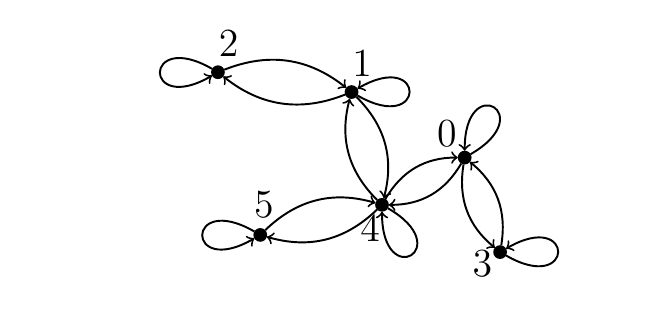
\begin{tikzpicture}[dot/.style={draw,circle,fill,inner sep=1.5pt},line width=.7pt,x=1.5cm,y=1.5cm]
\clip(-1,1.3) rectangle (4,3.5);
\begin{scriptsize}
\node (r0) at (2.7,2.4) [dot] {};
\draw[color=black] (2.55,2.6) node {{\Large $0$}};

\node (r1) at (1.7420645075484014,2.9548225063123694) [dot] {};
\draw[color=black] (1.8316581320147085,3.195605372065557) node {{\Large $1$}};


\node (r2) at (0.6109449986613309,3.1228105521866865) [dot] {};
\draw[color=black] (0.7005386231276353,3.363593417939874) node {{\Large $2$}};

\node (r3) at (3,1.6) [dot] {};
\draw[color=black] (2.85,1.5) node {{\Large $3$}};

\node (r4) at (2,2) [dot] {};
\draw[color=black] (1.9,1.8) node {{\Large $4$}};

\node (r5) at (0.9693194965265414,1.7453085760172875) [dot] {};
\draw[color=black] (1,2) node {{\Large $5$}};

\draw[->] (r0) to[out=30,in=90,looseness=30] (r0);
\draw[->] (r1) to[out=-30,in=30,looseness=30] (r1);
\draw[->] (r2) to[out=150,in=210,looseness=30] (r2);
\draw[->] (r3) to[out=-30,in=30,looseness=30] (r3);
\draw[->] (r4) to[out=-30,in=-90,looseness=30] (r4);
\draw[->] (r5) to[out=150,in=210,looseness=30] (r5);

\draw[->] (r0) to[bend left] (r4);
\draw[->] (r4) to[bend left] (r0);

\draw[->] (r0) to[bend right] (r3);
\draw[->] (r3) to[bend right] (r0);

\draw[->] (r5) to[bend left] (r4);
\draw[->] (r4) to[bend left] (r5);

\draw[->] (r1) to[bend left] (r4);
\draw[->] (r4) to[bend left] (r1);

\draw[->] (r1) to[bend left] (r2);
\draw[->] (r2) to[bend left] (r1);

\end{scriptsize}
\end{tikzpicture}
%\end{document}

\end{figure}
    {\large 11~12~22~21~11~{\red 14}~44~45~55~54~44~40~00~04~44~43~33~34~44~{\red 41~11}}
\end{center}
\end{frame}

\begin{frame}{Euler Tour Trees}

\begin{figure}[htb]
\centering
\scalebox{.7}{
\input{fig/SEQ-INDICES.tex}}
\end{figure}
\begin{center}
{\large 11~12~22~21~11~14~44~45~55~54~44~40~00~04~44~43~33~34~44~41~11}

\end{center}
\end{frame}



\begin{frame}{Chaves implícitas}
\begin{figure}[htb]
\scalebox{.7}{
\centering
\input{fig/SEQ-SIZE.tex}}
\end{figure}
\begin{center}
{\large 11~12~22~21~11~14~44~45~55~54~44~40~00~04~44~43~33~34~44~41~11}
\end{center}
\end{frame}


\begin{frame}{Biblioteca de Euler Tour Trees}
\begin{exampleblock}{Biblioteca de Euler Tour Trees}
\begin{itemize}
\item  \treapCreate(\var{u},\var{v}): retorna uma ABB com um único nó com valor uv;
\item \treapJoin(\var{T},\var{R}): junta as ABBs \var{T} e \var{R} concatenando as sequências Eulerianas armazenada nelas e retorna a raiz da árvore resultante.
\item \treapSplit(\var{T},\var{node}): corta~\var{T} em duas ABBs. A primeira contendo todos os nós anteriores a~\var{node} e a segunda os demais;
\item \treapGetRoot(\var{x}): retorna a raiz da ABB que contém \var{x};
\item \treapSearch(\var{T},\var{k}): retorna o nó com chave \var{k} da árvore \var{T};
\item \treapOrder(\var{node}): retorna a chave de \var{node};
\item \treapGetLast(\var{T}): retorna o nó de maior chave na árvore~\var{T}; e
\item \treapGetSize(\var{T}): retorna o número de nós em \var{T}.
\end{itemize}
\end{exampleblock}
\boxpurple{\centering  \treapCreate{} e \treapGetSize{} :~$\O{1}$.\\ As demais operações :~$\O{\lg n}$.}
\end{frame}


\begin{frame}{Tabela de símbolos}
\boxblue{
\centering
Associa \var{(u,v)} $\rightarrow$ \var{uv}.
}
\begin{exampleblock}{Biblioteca de tabela de símbolos}
    \begin{itemize}
    \item \hashCreate(\var{n}): retorna uma tabela hash para armazenar valores associados a valores em \var{n}$\times$\var{n};
    \item \hashAdd(\dymForestHash{},\var{u},\var{v},\var{uv}): associa o par \var{(u,v)} à~\var{uv} em~\dymForestHash{};
    \item \hashDel(\dymForestHash{},\var{u},\var{v}): remove o conteúdo associado ao par~\var{(u,v)} de~\dymForestHash{};
    \item \hashGet(\dymForestHash{},\var{u},\var{v}): retorna o valor associado ao par~\var{(u,v)} da tabela~\dymForestHash{}.
\end{itemize}
\end{exampleblock}
\boxpurple{
\centering
Consumo esperado~$\O{1}$ por rotina~\cite{CLRS}.
}
\end{frame}



\begin{frame}{Implementação da interface de floresta dinâmica}

\begin{algorithm}[H]
\caption{\dymForestCreate(\var{n})}
\label{Algo:dymForestCreate}
\begin{algorithmic}[1]
\State \var{F}.\var{n} $\gets$ \var{n}
\State \var{F}.\dymForestHash{} $\gets$ \hashCreate(\var{n})
\For {\var{v} $\gets$ 1 até \var{n}}\label{Algo:dymForestCreate:for}
\State \hashAdd(\var{F}.\dymForestHash{},\var{v},\var{v},\treapCreate(\var{v},\var{v}))
\EndFor
\State \Return \var{F}
\end{algorithmic}
\end{algorithm}
\begin{algorithm}[H]
\caption{\dymForestQuery(\var{F},\var{u},\var{v})}
\label{Algo:dymForestQuery}
\begin{algorithmic}[1]
\State \var{uu} $\gets$ \hashGet(\var{F}.\dymForestHash,\var{u},\var{u})
\State \var{vv} $\gets$ \hashGet(\var{F}.\dymForestHash,\var{v},\var{v})
\State \Return \treapGetRoot(\var{uu}) = \treapGetRoot(\var{vv})
\end{algorithmic}
\end{algorithm}
\boxpurple{
\centering
~~~~~\dymForestCreate{} : $\O{n}$\\
\dymForestQuery{}  : $\O{\lg n}$
}
\end{frame}

\begin{frame}{Implementação da interface de floresta dinâmica}
\begin{algorithm}[H]
\caption{\dymForestAddEdge(\var{F},\var{u},\var{v})}
\label{Algo:dymForestAddEdge}
\begin{algorithmic}[1]
\State \ETmovetofront(\var{F},\var{u})
\State \ETmovetofront(\var{F},\var{v})
\State \var{U} $\gets$ \treapGetRoot(\hashGet(\var{F}.\dymForestHash,\var{u},\var{u}))
\State \var{V} $\gets$ \treapGetRoot(\hashGet(\var{F}.\dymForestHash,\var{v},\var{v}))
\State \var{uv} $\gets$ \treapCreate(\var{u},\var{v})
\State \var{vu} $\gets$ \treapCreate(\var{v},\var{u})
\State \var{uu} $\gets$ \treapCreate(\var{u},\var{u})
\State \hashAdd(\var{F}.\dymForestHash{},\var{u},\var{v},\var{uv})
\State \hashAdd(\var{F}.\dymForestHash{},\var{v},\var{u},\var{vu})
\State \treapJoin(\treapJoin(\treapJoin(\treapJoin(\var{U},\var{uv}),\var{V}),\var{vu}),\var{uu})\end{algorithmic}
\end{algorithm}
\boxpurple{
\centering
\dymForestAddEdge{}  : $\O{\lg n}$
}
\end{frame}

\begin{frame}{Rotina auxiliar \ETmovetofront{}}
\begin{algorithm}[H]
\caption{\ETmovetofront(\var{F},\var{u})}
\label{Algo:ETmovetofront}
\begin{algorithmic}[1]
\State \var{uu} $\gets$ \hashGet(\var{F}.\dymForestHash,\var{u},\var{u})
\State \var{T} $\gets$ \treapGetRoot(\var{uu})
\State \var{vv} $\gets$ \treapSearch(\var{T},1)
\If {\var{vv} $\neq$ \var{uu}} 
\State \hashAdd(\var{F}.\dymForestHash{},\var{v},\var{v},\var{vv}) 
\State \var{A}, \var{B} $\gets$ \treapSplit(\var{T}, \var{uu})
\State \var{vv} $\gets$ \treapGetLast(\var{B})
\State \var{B}, \var{C} $\gets$ \treapSplit(\var{T}, \var{vv})
\State \var{uu} $\gets$ \treapCreate(\var{u},\var{u})
\State \treapJoin(\treapJoin(\var{B},\var{A}),\var{uu})
\EndIf
\end{algorithmic}
\end{algorithm}
\boxpurple{
\centering
\ETmovetofront{}  : $\O{\lg n}$
}
\end{frame}

\begin{frame}{Implementação da interface de floresta dinâmica}
\begin{algorithm}[H]
\caption{\dymForestDelEdge(\var{F},\var{u},\var{v})}
\label{Algo:dymForestDelEdge}
\begin{algorithmic}[1]
\State \var{Kuv} $\gets$ \treapOrder(\hashGet(\var{F}.\dymForestHash{},\var{u},\var{v}))
\State \var{Kvu} $\gets$ \treapOrder(\hashGet(\var{F}.\dymForestHash{},\var{v},\var{u})) 
\If {\var{Kuv} $>$ \var{Kvu}}
	\Comment{garante que \var{uv} aparece na sequência antes de \var{vu}}
	\State \var{u} $\leftrightarrow$ \var{v}
	\State \var{Kuv} $\leftrightarrow$ \var{Kvu}
\EndIf
\State \var{S} $\gets$ \treapGetRoot(\var{uv})
\State \var{uu} $\gets$ \treapSearch(\var{S},\var{Kuv}-1)\Comment{obtém a ocorrência de \var{uu} que precede \var{uv}}
\State \var{vv} $\gets$ \treapSearch(\var{S},\var{Kuv}+1)
\State \var{A}, \var{B} $\gets$ \treapSplit(\var{S}, \var{uu})
\State \var{B}, \var{C} $\gets$ \treapSplit(\var{B}, \var{vv})
\State \var{C}, \var{D} $\gets$ \treapSplit(\var{B}, \var{vu})
\State \var{uu} $\gets$ \treapSearch(\var{D},2)
\State \var{D}, \var{E} $\gets$ \treapSplit(\var{D}, \var{uu})
\State \hashAdd(\var{F}.\dymForestHash{},\var{u},\var{u},\var{uu})
\State \hashDel(\var{F}.\dymForestHash{},\var{u},\var{v})
\State \hashDel(\var{F}.\dymForestHash{},\var{v},\var{u})
\State \treapJoin(\var{A},\var{E})
\end{algorithmic}
\end{algorithm}
\boxpurple{
\centering
\dymForestDelEdge{}  : $\O{\lg n}$
}
\end{frame}

\subsection{Treaps}
\begin{frame}{Uma treap imersa no plano cartesiano.}
\boxblue{
\centering
Cada nó da treap possui um par ordenado \textbf{(chave,prioridade)}

}
\begin{figure}[htb]
\centering
\scalebox{.45}{
\input{fig/TREAP.tex}}
\end{figure}
\end{frame}

\section{Conexidade em grafos dinâmicos}
\begin{frame}{Conexidade em grafos dinâmicos}
\begin{exampleblock}{Conexidade em grafos dinâmicos}
\begin{itemize}
\item \dymGraphCreate(\var{n}): cria um grafo dinâmico com \var{n} vértices isolados;
\item \dymGraphAddEdge(\var{G},\var{u},\var{v}): adiciona a aresta \var{uv} ao grafo dinâmico \var{G};
\item \dymGraphDelEdge(\var{G},\var{u},\var{v}): remove a aresta \var{uv} de \var{G}; e
\item \dymGraphQuery(\var{G},\var{u},\var{v}): retorna verdadeiro se \var{u} e \var{v} estão na mesma componente conexa de \var{G} e falso, caso contrário.
\end{itemize}
\end{exampleblock}

\end{frame}

\begin{frame}{Ideia inicial}
\begin{block}{Manteremos}
\begin{itemize}
    \item floresta maximal dinâmica~\var{F} de~\var{G}; e
    \item um grafo~\var{R} = $\var{G}-\var{F}$
\end{itemize}
\end{block}

\begin{exampleblock}{Lista de adjacências}
\begin{itemize}
    \item \graphCreate(\var{n}): devolve a representação por listas de adjacências de um grafo com~\var{n} vértices isolados.
    \item \graphAdd(\var{G},\var{u},\var{v}): adiciona \var{u} na lista de adjacências de \var{v} em \var{G} e vice-versa.
    \item \graphDel(\var{G},\var{u},\var{v}): remove \var{u} da lista de adjacências de \var{v} em \var{G} e vice-versa.
\end{itemize}
\end{exampleblock}
\boxpurple{
\centering
~~~~~~\graphCreate{} : $\O{\var{n}}$\\
\graphAdd{}  : $\O{1}$\\
\graphDel{}  : $\O{1}$\\
}
\end{frame}


\begin{frame}{Ideia inicial}
\begin{algorithm}[H]
\caption{\dymGraphQuery(\var{G},\var{u},\var{v})}
\label{Algo:dymGraphQuery}
\begin{algorithmic}[1]
\State \Return \dymForestQuery(\var{G}.\var{F},\var{u},\var{v})
\end{algorithmic}
\end{algorithm}
\begin{algorithm}[H]
\caption{\dymGraphAddEdge(\var{G},\var{u},\var{v})}
\label{Algo:dymGraphAddEdge}
\begin{algorithmic}[1]
\If {\dymForestQuery(\var{G}.\var{F},\var{u},\var{v})}
\State \graphAdd(\var{G}.\var{R},\var{u},\var{v})
\Else 
\State \dymForestAddEdge(\var{G}.\var{F},\var{u},\var{v})
\EndIf
\end{algorithmic}
\end{algorithm}
\boxpurple{
\dymGraphQuery{} : $\O{\lg n}$\\
\dymGraphAddEdge{}  : $\O{\lg^2 n}$ amortizado\TODO{!!}
}
\end{frame}



\begin{frame}{Remoção de arestas}
\begin{block}{Estrutura de níveis}
\begin{itemize}
    \item Cada aresta possui um \defi{nível}, que é um inteiro entre~$1$ e $\lceil \log \var{n} \rceil$;
    \item Arestas serão inseridas no nível~$\lceil \log \var{n} \rceil$;
    \item O nível de uma aresta pode diminuir, mas nunca aumentar. 
\end{itemize}
\end{block}
\begin{block}{Estrutura}
$\var{G}_\var{i}$: grafo com arestas de nível $\leqslant$ \var{i}. Para cada camada \var{i}, manteremos:
\begin{itemize}
    \item $\var{F}_\var{i}$: floresta maximal  de~$\var{G}_\var{i}$; e
    \item $\var{R}_\var{i}$: arestas de nível~\var{i} $\notin \var{F}_\var{i}$.
\end{itemize}
\end{block}
\begin{block}{Invariantes}
\begin{itemize}
    \item $\var{F}_\var{i}\subseteq \var{F}_{\var{i}+1}$, para cada $ 1\leqslant \var{i} \leqslant \lceil \log \var{n} \rceil-1$ e que $\var{F}_\var{i}$ é uma floresta maximal de~$\var{G}_\var{i}$; e
    \item Cada componente de $\var{F}_\var{i}$ possui menos do que $2^\var{i}$ arestas.
\end{itemize}
\end{block}
\end{frame}

\begin{frame}{Implementações}
\begin{exampleblock}{Adaptações}
\centering
$\var{G}.\var{F}\rightarrow\var{G}.\var{F}[\lceil \log \var{n} \rceil]$\\
$\var{G}.\var{R}\rightarrow\var{G}.\var{R}[\lceil \log \var{n} \rceil]$
\end{exampleblock}
\begin{algorithm}[H]
\caption{\dymGraphDelEdge(\var{G},\var{u},\var{v})}
\label{Algo:dymGraphDelEdge}
\begin{algorithmic}[1]
\If {\var{uv} $\in \var{G}.\var{F}[{\lceil \log \var{n} \rceil}]$}
\For {\var{i} $\gets$ \var{uv}.\var{nível} até $\lceil \log \var{n} \rceil$}\label{linha2}
\State \dymForestDelEdge(\var{G}.\var{F}[i],\var{u},\var{v}))
\EndFor
\State \dymGraphReplace(\var{G},\var{u},\var{v},\var{uv}.\var{nível})
\Else
  \State \graphDel(\var{G}.\var{R}[\var{uv}.\var{nível}],\var{u},\var{v})
\EndIf
\end{algorithmic}
\end{algorithm}
\boxpurple{
\centering
\dymGraphDelEdge{}  : $\O{\lg^2 \var{n}}$ amortizado
}
\end{frame}

\begin{frame}{Estrutura de níveis}
\begin{figure}[htb]
\scalebox{.5}{
\input{fig/antes-rebaixar}
\begin{tikzpicture}[line cap=round,line join=round,x=1cm,y=1cm]
\clip(0,-.5) rectangle (5,4.5);
\end{tikzpicture}
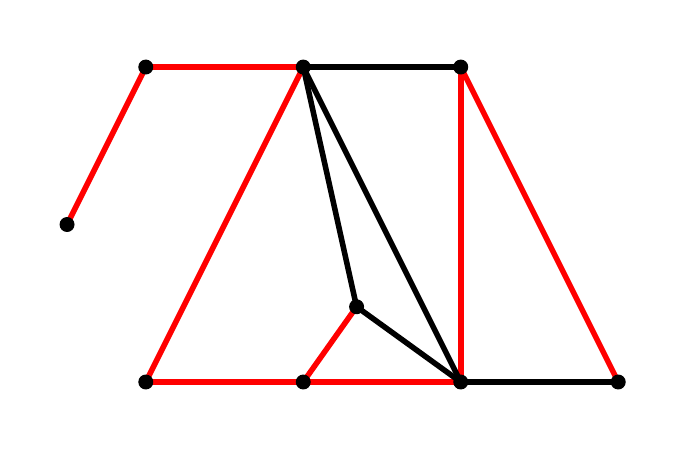
\begin{tikzpicture}[line cap=round,line join=round,x=1cm,y=1cm]
\clip(-.5,-.5) rectangle (7.5,4.5);
\draw [line width=2pt,color=ccqqqq] (3,0)-- (3.677138935355088,0.9555967043150745);
\draw [line width=2pt,color=ccqqqq] (3,0)-- (1,0);
\draw [line width=2pt,color=ccqqqq] (3,0)-- (5,0);
\draw [line width=2pt,color=ccqqqq] (5,0)-- (5,4);
\draw [line width=2pt,color=ccqqqq] (1,4)-- (3,4);
\draw [line width=2pt] (3,4)-- (5,0);
\draw [line width=2pt] (3.677138935355088,0.9555967043150745)-- (5,0);
\draw [line width=2pt] (5,4)-- (3,4);
\draw [line width=2pt,color=ccqqqq] (1,4)-- (0,2);
\draw [line width=2pt,color=ccqqqq] (1,0)-- (3,4);
\draw [line width=2pt] (3,4)-- (3.677138935355088,0.9555967043150745);
\draw [line width=2pt,color=ccqqqq] (5,4)-- (7,0);
\draw [line width=2pt] (7,0)-- (5,0);
\begin{scriptsize}
\draw [fill=black] (3,0) circle (2.5pt);
\draw [fill=black] (3.677138935355088,0.9555967043150745) circle (2.5pt);
\draw [fill=black] (1,0) circle (2.5pt);
\draw [fill=black] (1,4) circle (2.5pt);
\draw [fill=black] (0,2) circle (2.5pt);
\draw [fill=black] (3,4) circle (2.5pt);
\draw [fill=black] (5,0) circle (2.5pt);
\draw [fill=black] (5,4) circle (2.5pt);
\draw [fill=black] (7,0) circle (2.5pt);
\end{scriptsize}
\end{tikzpicture}}
\end{figure}
\begin{figure}[htb]
\scalebox{.5}{
\input{fig/pontos}
\begin{tikzpicture}[line cap=round,line join=round,x=1cm,y=1cm]
\clip(0,-.5) rectangle (5,4.5);
\end{tikzpicture}
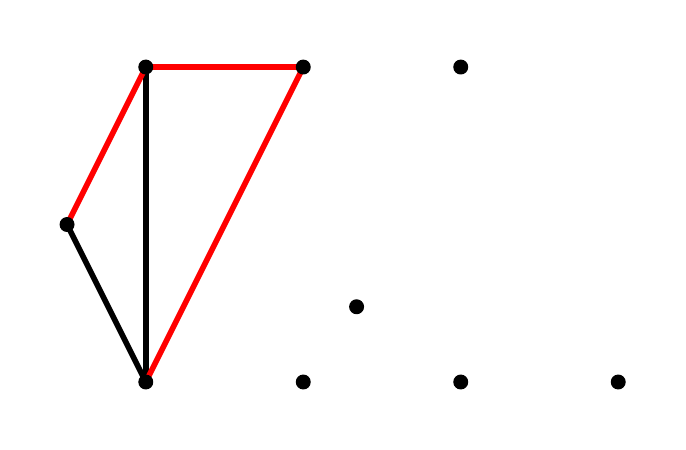
\begin{tikzpicture}[line cap=round,line join=round,x=1cm,y=1cm]
\clip(-.5,-.5) rectangle (7.5,4.5);
\draw [line width=2pt] (1,0)-- (1,4);
\draw [line width=2pt] (1,0)-- (0,2);
\draw [line width=2pt,color=ccqqqq] (1,4)-- (3,4);
\draw [line width=2pt,color=ccqqqq] (1,4)-- (0,2);
\draw [line width=2pt,color=ccqqqq] (1,0)-- (3,4);
\begin{scriptsize}
\draw [fill=black] (3,0) circle (2.5pt);
\draw [fill=black] (3.677138935355088,0.9555967043150745) circle (2.5pt);
\draw [fill=black] (1,0) circle (2.5pt);
\draw [fill=black] (1,4) circle (2.5pt);
\draw [fill=black] (0,2) circle (2.5pt);
\draw [fill=black] (3,4) circle (2.5pt);
\draw [fill=black] (5,0) circle (2.5pt);
\draw [fill=black] (5,4) circle (2.5pt);
\draw [fill=black] (7,0) circle (2.5pt);
\end{scriptsize}
\end{tikzpicture}}
\end{figure}
\end{frame}




\begin{frame}{A rotina \dymGraphReplace{}}

\begin{algorithm}[H]
\caption{\dymGraphReplace(\var{G},\var{u},\var{v},\var{nível})}
\label{Algo:dymGraphReplace}
\begin{algorithmic}[1]
\For {\var{i} $\gets$ \var{nível} até $\lceil \log \var{n} \rceil$}\label{Algo:dymGraphReplace:linha:primeira}
\State $\var{T}_\var{v}$ $\gets$  \treapGetRoot(\hashGet(\var{G}.\var{F}[\var{i}].\dymForestHash,\var{v},\var{v}))
\State $\var{T}_\var{u}$ $\gets$  \treapGetRoot(\hashGet(\var{G}.\var{F}[\var{i}].\dymForestHash,\var{u},\var{u}))
\If {$\treapGetSize(\var{T}_\var{v}) < \treapGetSize(\var{T}_\var{u})$}\Comment{Garantimos que $|\var{T}_\var{v}|\geqslant |\var{T}_\var{u}|$}
\State \var{u} $\leftrightarrow$ \var{v}
\State $\var{T}_\var{u} \leftrightarrow \var{T}_\var{v}$
\EndIf
\For {\var{xy} em $\var{T}_\var{u}$ com \var{xy}.\var{nível} = \var{i}}\label{Algo:dymGraphReplace:linha:moveTu}\Comment{Move $\var{T}_\var{u}$ para o nível \var{i-1}}
\State \var{xy}.\var{nível} $\gets$ \var{i} $-$ 1
\State \dymForestAddEdge(\var{G}.\var{F}[\var{i}-1],\var{x},\var{y}) 
\EndFor
\For {\var{xy} em \var{G}.\var{R}[\var{i}] com \var{x} em $\var{T}_\var{u}$}\label{Algo:dymGraphReplace:linha:achaSub}\Comment{Procura substituta para \var{uv}}
\State \graphDel(\var{G}.\var{R}[\var{i}],\var{x},\var{y})
\If {\var{y} $\in \var{T}_\var{v}$}
\For {\var{j} $\gets$ \var{i} até $\lceil \log \var{n} \rceil$}
\State \dymForestAddEdge(\var{G}.\var{F}[\var{j}],\var{x},\var{y})
\EndFor
\Return
\Else
\State \var{xy}.\var{nível} $\gets$ \var{i} $-$ 1
\State \graphAdd(\var{G}.\var{R}[\var{i} - 1],\var{x},\var{y})
\EndIf
\EndFor
\EndFor\label{Algo:dymGraphReplace:linha:ultima}
\end{algorithmic}
\end{algorithm}
\end{frame}


\section{Floresta maximal de peso mínimo em grafos planos}

\begin{frame}{Floresta maximal de peso mínimo}
\begin{exampleblock}{O problema da floresta maximal de peso mínimo em grafos planos}
\begin{itemize}
\item \MSFCreate(\var{n}): devolve um grafo dinâmico com \var{n} vértices isolados;
\item \MSFaddEdge(\var{G},\var{u},\var{v},\var{w}): adiciona \var{uv} com peso \var{w} a~\var{G};
\item \MSFdelEdge(\var{G},\var{u},\var{v}): remove \var{uv} de~\var{G}; e
\item \MSFweight(\var{G}): devolve o peso de uma MSF de \var{G}.
\end{itemize}
\end{exampleblock}

\end{frame}


\begin{frame}{Caso decremental}
\begin{exampleblock}{O caso decremental do problema MSF em grafos ponderados dinâmicos}
\begin{itemize}
\item \MSFCreate(\var{H}): recebe um grafo~\var{H} e devolve um grafo dinâmico e uma MSF dele;
\item \MSFdelEdge(\var{G},\var{u},\var{v}): remove \var{uv} de~\var{G}; e
\item \MSFweight(\var{G}): devolve o peso de uma MSF de \var{G}.
\end{itemize}
\end{exampleblock}
\begin{exampleblock}{Adaptação para o caso decremental}
\begin{itemize}
    \item $\var{F}_{\lceil \log \var{n} \rceil}$ deve ser de peso mínimo;
    \item Em \dymGraphReplace{}, percorrer as arestas de nível \var{i} em ordem crescente de peso;
\end{itemize}
\end{exampleblock}
\end{frame}

\iffalse
\begin{frame}{Caso decremental}
\begin{algorithm}[H]
\caption{\MSFCreate(\var{H})}
\begin{algorithmic}[1]
\State \var{G} $\gets$ \dymGraphCreate($|\var{H}|$)
\State \var{F} $\gets$ Encontre uma MSF de \var{H}\Comment{Podemos usar Kruskal ou Prim}
\For {\var{uv} $\in$ \var{F}}
\State \dymGraphAddEdge(\var{G},\var{u},\var{v}\TODO{,\var{uv.w}})
\EndFor
\For {\var{uv} $\in$ \var{H} e \var{uv} $\notin$ \var{F}}
\State \dymGraphAddEdge(\var{G},\var{u},\var{v}\TODO{,\var{uv.w}})
\EndFor
\State \Return \var{G}
\end{algorithmic}
\end{algorithm}

\end{frame}
\fi

\subsection{Rotina para adição de arestas}
\begin{frame}{Adição de arestas}
\begin{algorithm}[H]
\caption{\MSFaddEdge(\var{G},\var{u},\var{v},\var{w})}
\label{Algo:MSFaddEdge}
\begin{algorithmic}[1]
\If {\dymForestQuery(\var{G}.\var{F},\var{u},\var{v})}
  \For{cada \var{xy} no caminho de \var{u} a \var{v} em \var{G}.\var{F}}
  \If{\var{xy}.\var{w} > \var{w}}
  \State \dymForestDelEdge(\var{G}.\var{F},\var{x},\var{y})
  \State \dymForestAddEdge(\var{G}.\var{F},\var{u},\var{v}\TODO{,\var{w}})
  \State \Return
  \EndIf
  \EndFor
  \State \graphAdd(\var{G}.\var{R},\var{u},\var{v}\TODO{,\var{w}})
\Else
\State \dymForestAddEdge(\var{G}.\var{F},\var{u},\var{v}\TODO{,\var{w}})
\EndIf
\end{algorithmic}
\end{algorithm}
\begin{exampleblock}{Árvores topológicas}
 \defi{Árvores topológicas} (top tree)~\cite{AHLTMinDiameter} permitem:
    \begin{itemize}
        \item obter informação sobre conexidade; e
        \item percorrer caminhos da árvore.
    \end{itemize}
\end{exampleblock}
\end{frame}






\section{Bibliografia}
\begin{frame}[allowframebreaks]
\frametitle{Bibliografia}
\bibliographystyle{plain}
    \bibliography{bib.bib}

\end{frame}

\end{document}
